\section{CDrive}
CDrive is designed as a collection of microservices that communicate between each other. Each of 
these microservices are containierized and deployed on a Kubernetes cluster. Kubernetes connects 
these microservices over an internal network which they use for communicating among themselves.


\subsection{Authentication}
CDrive uses the Oauth 2.0 protocol for authentication and authorization. Oauth allows applications 
to access a user's CDrive data in a secure way once the user has given the application permission 
to do so. These are the steps that an application follows in order to access CDrive data:

\begin{itemize}
  \item Registration: An application needs to be registered in order to obtain a client id and a
    client secret. The registration process has some differences depending on the type of
    application (i.e. private, shared or hosted) but at the end of the process the application 
    receives a client id and a client secret.
  \item Authorization: Next, the application will require the user to authorize it to access some
    data within the user's CDrive.
  \item Access: Once the application has been authorized, the application receives a temporary code
    which it can use along with the client id and client secret to request an access token from 
    CDrive. CDrive uses the client id and client secret to verify the identity of the application 
    and sends it an access token. Using the access token, the application
    can access the user's CDrive data that it was authorized to access.
\end{itemize}

CDrive has an authentication microservice which exposes REST endpoints that applications 
can hit in order to carry out the Oauth workflow outlined above.

\subsection{Drive API}
CDrive exposes a Drive API microservice over the internet. The Drive API microservice defines REST
endpoints for CDrive actions such as upload, download, share, delete, create, list directories etc.
Once an application has obtained an access token as described in the previous section, the
application can hit these rest endpoints to modify CDrive data. CDrive internally communicates with
the authentication microservice to authenticate these requests based on the access token passed with
this request.

\begin{figure}[t]
  \caption{Routing in Columbus}
  \centering
  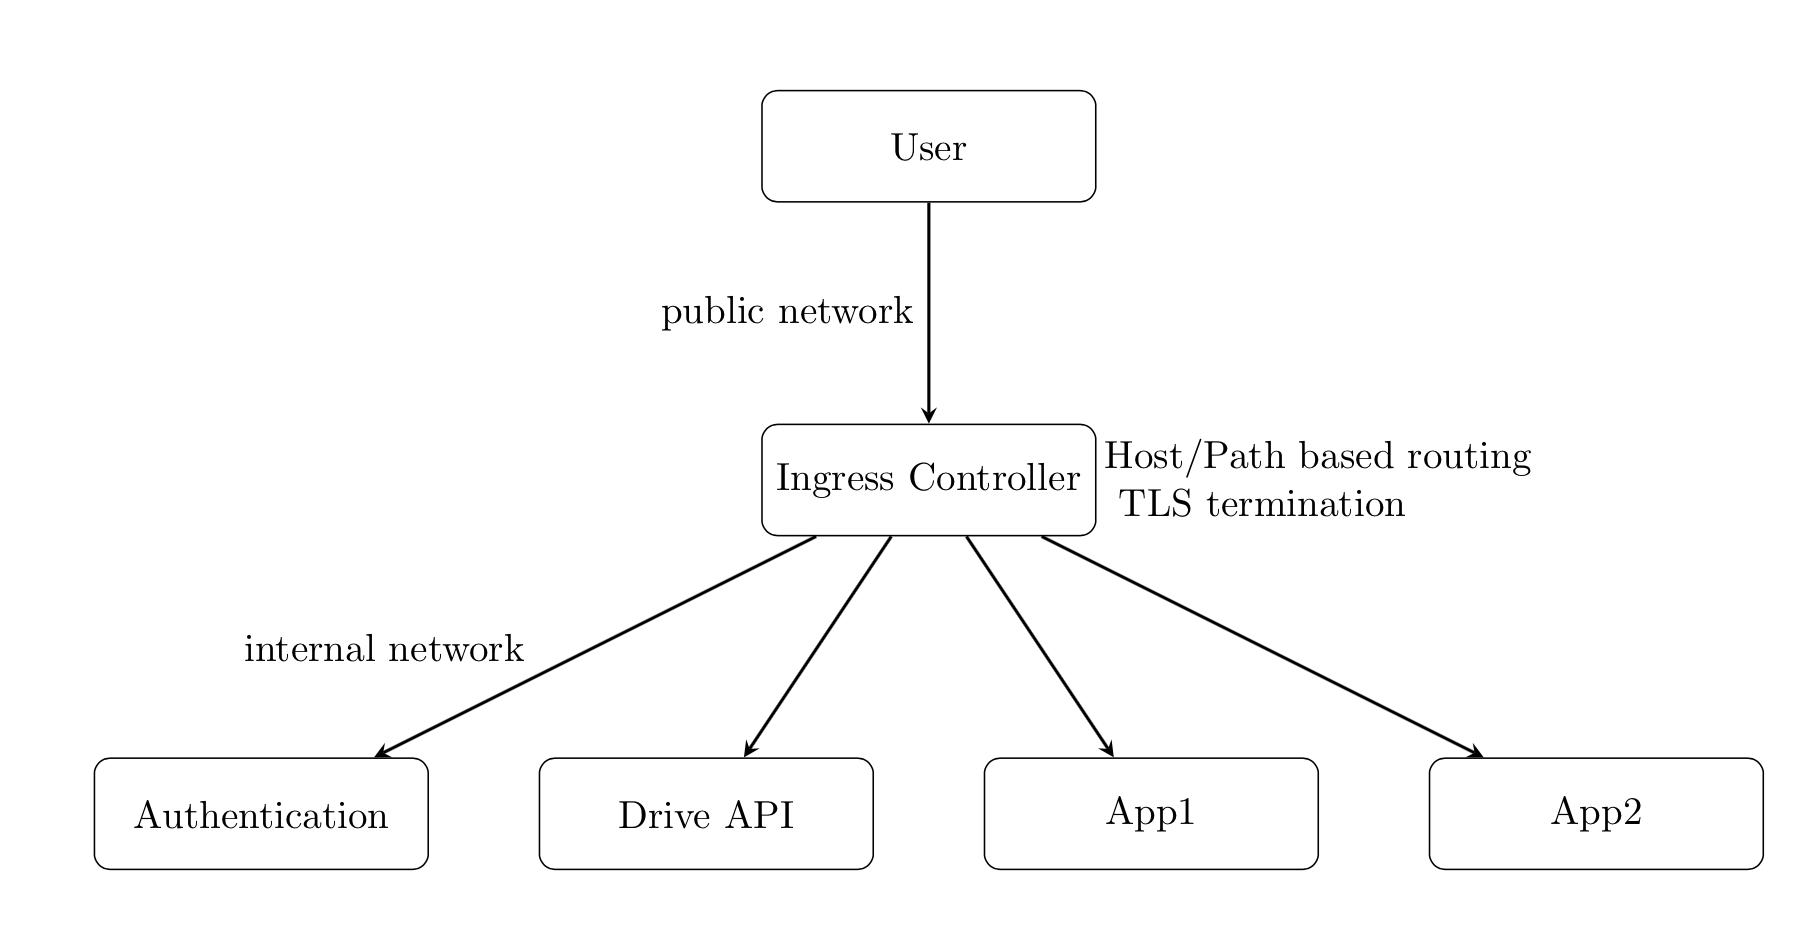
\includegraphics[width=9cm, height=5cm]{routing}
\end{figure}

\subsection{User interface}
CDrive has a user interface that allows users to create Columbus accounts, login and use Columbus.
The user interface is served from a set of containers running on Kubernetes pods. Kubernetes
balances the load between these pods. The user interface internally follows the procedured outlined
above to obtain an access token by making requests to the authentication microservice and then uses
that token to make API calls to the drive API to perform user actions. 

From the user interface, the user can:
\begin{itemize}
  \item Manage data on their account with actions such as upload, download, delete, share, edit etc.
  \item Install and use different applications to operate on the CDrive data.
  \item Use the Jupyter Notebook interface to programmatically access the CDrive API and the API 
    exposed by other applications.
\end{itemize}

\subsection{Ingress controller}
CDrive exposes some API endpoints such as drive APIs and authentication APIs over the internet. 
Also, the CDrive UI, private applications and shared applications are served from the Kubernetes 
cluster over the internet. We set up an ingress controller as the single end point to receive 
requests to any of the services running on the Kubernetes cluster. The ingress controller is 
responsible for routing these requests to appropriate services. A Kubernetes ingress object is 
created for each service. This object specifies the configuration rules that the ingress controller
should use for routing requests to the concerned service.


We use different domain or sub-domain names for different services such as authentication, drive api
, private applications and each shared application. We use virtual hosting to serve all these 
domains from a common endpoint. Virtual hosting is a method that allows multiple domains to be 
served by a common pool of servers or in our case, by a single common Kubernetes cluster. Virtual 
hosting allows services to share server resources such as memory and processor cycles without 
requiring all the services to use the same domain name. 


We add DNS A records for each of the domains the cluster will host and point all of these to the 
public IP address of the ingress controller service. Requests to any of these domains will now be
directed to the ingress controller. The ingress controller then uses a combination of hostname and
path to route the request to the appropriate service over the internal Kubernetes network. Hostname
based routing is used to route requests to the authentication service, drive api and all shared 
applications. All private applications are accessed under the same hostname. The username and 
application name are required to be specified in the path and path based routing is used to route 
these requests. For example, when user u-i installs app a-j, CDrive launches an instance of a-j
in a pod, exposes it within the cluster as a service and adds a Kubernetes ingress resource for it
which configures a reverse proxy for this app on the ingress controller. Subsequently, any request 
to APP-URL/u-i/a-j/... will be routed to user u-i's instance of app a-j by the ingress
controller.


Alongside routing, the ingress controller also provides TLS termination, thus allowing all services
to be served over HTTPS. The assumption here is that the Kubernetes internal network is secure. 
Given this assumption, it is useful to have TLS termination implemented in a central location 
instead of each service having to implement it separately. This is beneficial to Columbus app 
developers as well, as their apps avail the additional security layer of HTTPS without the
additional development effort of imlementing TLS termination.


Columbus uses Cert-Manager, Kubernetes’ native certificate manager to automatically provision TLS
certificates. We create a Cluster Issuer resource for issuing certificates. The Cert-Manager
contacts the Cluster Issuer to request TLS certificates. The Cluster Issuer resource represents a
certificate authority. The Columbus Cluster Issuer is configured to use TLS certificates from
Let’s Encrypt, which is a free, automated and open certificate authority. 

\subsection{Persistent storage}
Kubernetes, by default, runs containers as 'stateless' pods i.e. Kubernetes assumes that the 
containers do not have any persistent data within them. In such a scenario, whenever Kubernetes 
shuts down an application container and starts a new container, application data will be lost. 
Kubernetes is designed to do this occasionally for load balancing and several other reasons.


This problem is typically addressed on Kubernetes using a concept called 'Stateful Sets'.  
Applications configured as stateful sets, will attach a Kubernetes persistent volume to pods. 
These persistent volumes will last beyond the lifecycle of the pod, and any new pods for the 
application will connect to this persistent volume to recover state. Kubernetes persistent volumes 
are similar to docker volume mounts. But where Docker only allows mounting a volume to a host 
directory, Kubernetes offers various other alternatives such as EBS Volumes, NFS, Cephfs, Glusterfs,
EFS etc.


In Columbus, we attach EBS Volumes to application pods as persistent volumes using a Persistent 
Volume Claim. This storage is dynamic in the sense that if a persistent volume is not bound to 
persistent volume claim, a new EBS volume is dynamically provisioned and bound to it. If a 
persistent volume is already bound to the claim, the stateful application attaches to it. So, 
Kubernetes can shut down and re-start these container many times but the data is always maintained 
as the same EBS volume is always re-attached.

\subsection{App manager}
CDrive's app manager microservice exposes a set of API endpoints internally on the Kubernetes
cluster. The app manager service is responsible for installing, pausing, re-starting and deleting 
private applications and exposes API endpoints for these tasks. The app manager configures all the
Kubernetes resources such as deployments, services, ingresses and persistent volumes which are 
required to pull and run the docker image of an application. The app manager does so by 
communicating with the Kubernetes cluster using the Kubernetes API. The app manager is the only 
microservice on the cluster that is authorized to use the Kubernetes API.
